
\documentclass[11pt,a4paper,oneside]{report}

\usepackage{float}
\usepackage{tikz}
\usetikzlibrary{plotmarks}
\usepackage{amsmath,graphicx}
\usepackage{epstopdf}
\usepackage[font=normal,labelfont=bf]{caption}
\usepackage{subcaption}
\usepackage{color}
\usepackage[T1]{fontenc}
\usepackage{lmodern}
\usepackage{scalefnt}


% margin size
\usepackage[margin=1in]{geometry}

% tikz settings
\tikzstyle{state}=[circle,thick,draw=black, align=center, minimum size=2.1cm,
inner sep=0]
\tikzstyle{vertex}=[circle,thick,draw=black]
\tikzstyle{terminal}=[rectangle,thick,draw=black]
\tikzstyle{edge} = [draw,thick]
\tikzstyle{lo} = [edge,dotted]
\tikzstyle{hi} = [edge]
\tikzstyle{trans} = [edge,->]


\begin{document}
\belowdisplayskip=12pt plus 3pt minus 9pt
\belowdisplayshortskip=7pt plus 3pt minus 4pt

% scale parameter for the circles and the gradient
\tikzset{every picture/.append style={scale=0.6}}
% scale parameter for the upper and lower small brain images
\newcommand*{\scaleBrainImg}{0.3}

%col{x}{y}{z} respresents the color for ball z from matrix x at stage y (matrix x, stage y, ball z)

\definecolor{col000}{rgb}{1,0.000,0}
\definecolor{col001}{rgb}{1,0.000,0}
\definecolor{col002}{rgb}{1,0.000,0}
\definecolor{col003}{rgb}{1,0.000,0}
\definecolor{col004}{rgb}{1,0.000,0}
\definecolor{col005}{rgb}{1,0.000,0}
\definecolor{col006}{rgb}{1,1.000,0}
\definecolor{col010}{rgb}{1,0.000,0}
\definecolor{col011}{rgb}{1,0.000,0}
\definecolor{col012}{rgb}{1,0.000,0}
\definecolor{col013}{rgb}{1,0.000,0}
\definecolor{col014}{rgb}{1,0.000,0}
\definecolor{col015}{rgb}{1,0.000,0}
\definecolor{col016}{rgb}{1,0.928,0}
\definecolor{col020}{rgb}{1,0.000,0}
\definecolor{col021}{rgb}{1,0.000,0}
\definecolor{col022}{rgb}{1,0.000,0}
\definecolor{col023}{rgb}{1,0.000,0}
\definecolor{col024}{rgb}{1,0.000,0}
\definecolor{col025}{rgb}{1,0.000,0}
\definecolor{col026}{rgb}{1,0.000,0}
\definecolor{col030}{rgb}{1,0.000,0}
\definecolor{col031}{rgb}{1,0.000,0}
\definecolor{col032}{rgb}{1,0.000,0}
\definecolor{col033}{rgb}{1,0.000,0}
\definecolor{col034}{rgb}{1,0.000,0}
\definecolor{col035}{rgb}{1,0.000,0}
\definecolor{col036}{rgb}{1,0.000,0}
\definecolor{col040}{rgb}{1,0.000,0}
\definecolor{col041}{rgb}{1,0.000,0}
\definecolor{col042}{rgb}{1,0.000,0}
\definecolor{col043}{rgb}{1,0.000,0}
\definecolor{col044}{rgb}{1,0.000,0}
\definecolor{col045}{rgb}{1,0.000,0}
\definecolor{col046}{rgb}{1,0.000,0}
\definecolor{col100}{rgb}{1,0.000,0}
\definecolor{col101}{rgb}{1,0.000,0}
\definecolor{col102}{rgb}{1,0.251,0}
\definecolor{col103}{rgb}{1,0.000,0}
\definecolor{col104}{rgb}{1,0.000,0}
\definecolor{col105}{rgb}{1,0.000,0}
\definecolor{col106}{rgb}{1,0.938,0}
\definecolor{col110}{rgb}{1,0.000,0}
\definecolor{col111}{rgb}{1,0.000,0}
\definecolor{col112}{rgb}{1,0.000,0}
\definecolor{col113}{rgb}{1,0.000,0}
\definecolor{col114}{rgb}{1,0.000,0}
\definecolor{col115}{rgb}{1,0.000,0}
\definecolor{col116}{rgb}{1,0.287,0}
\definecolor{col120}{rgb}{1,0.000,0}
\definecolor{col121}{rgb}{1,0.000,0}
\definecolor{col122}{rgb}{1,0.000,0}
\definecolor{col123}{rgb}{1,0.000,0}
\definecolor{col124}{rgb}{1,0.000,0}
\definecolor{col125}{rgb}{1,0.000,0}
\definecolor{col126}{rgb}{1,0.041,0}
\definecolor{col130}{rgb}{1,0.000,0}
\definecolor{col131}{rgb}{1,0.000,0}
\definecolor{col132}{rgb}{1,0.000,0}
\definecolor{col133}{rgb}{1,0.000,0}
\definecolor{col134}{rgb}{1,0.000,0}
\definecolor{col135}{rgb}{1,0.000,0}
\definecolor{col136}{rgb}{1,-0.000,0}
\definecolor{col140}{rgb}{1,0.000,0}
\definecolor{col141}{rgb}{1,0.000,0}
\definecolor{col142}{rgb}{1,0.000,0}
\definecolor{col143}{rgb}{1,0.000,0}
\definecolor{col144}{rgb}{1,0.000,0}
\definecolor{col145}{rgb}{1,0.000,0}
\definecolor{col146}{rgb}{1,-0.000,0}
\definecolor{col200}{rgb}{1,0.000,0}
\definecolor{col201}{rgb}{1,0.020,0}
\definecolor{col202}{rgb}{1,0.020,0}
\definecolor{col203}{rgb}{1,0.050,0}
\definecolor{col204}{rgb}{1,-0.000,0}
\definecolor{col205}{rgb}{1,0.020,0}
\definecolor{col206}{rgb}{1,0.940,0}
\definecolor{col210}{rgb}{1,0.000,0}
\definecolor{col211}{rgb}{1,0.000,0}
\definecolor{col212}{rgb}{1,0.000,0}
\definecolor{col213}{rgb}{1,0.000,0}
\definecolor{col214}{rgb}{1,-0.000,0}
\definecolor{col215}{rgb}{1,0.000,0}
\definecolor{col216}{rgb}{1,0.010,0}
\definecolor{col220}{rgb}{1,0.000,0}
\definecolor{col221}{rgb}{1,0.000,0}
\definecolor{col222}{rgb}{1,0.000,0}
\definecolor{col223}{rgb}{1,0.000,0}
\definecolor{col224}{rgb}{1,-0.000,0}
\definecolor{col225}{rgb}{1,0.000,0}
\definecolor{col226}{rgb}{1,0.000,0}
\definecolor{col230}{rgb}{1,0.000,0}
\definecolor{col231}{rgb}{1,0.000,0}
\definecolor{col232}{rgb}{1,0.000,0}
\definecolor{col233}{rgb}{1,0.000,0}
\definecolor{col234}{rgb}{1,-0.000,0}
\definecolor{col235}{rgb}{1,0.000,0}
\definecolor{col236}{rgb}{1,0.000,0}
\definecolor{col240}{rgb}{1,0.000,0}
\definecolor{col241}{rgb}{1,0.000,0}
\definecolor{col242}{rgb}{1,0.000,0}
\definecolor{col243}{rgb}{1,0.000,0}
\definecolor{col244}{rgb}{1,-0.000,0}
\definecolor{col245}{rgb}{1,0.000,0}
\definecolor{col246}{rgb}{1,0.000,0}
\definecolor{col300}{rgb}{1,0.020,0}
\definecolor{col301}{rgb}{1,0.200,0}
\definecolor{col302}{rgb}{1,0.370,0}
\definecolor{col303}{rgb}{1,0.150,0}
\definecolor{col304}{rgb}{1,0.110,0}
\definecolor{col305}{rgb}{1,0.130,0}
\definecolor{col306}{rgb}{1,0.970,0}
\definecolor{col310}{rgb}{1,0.000,0}
\definecolor{col311}{rgb}{1,0.030,0}
\definecolor{col312}{rgb}{1,0.230,0}
\definecolor{col313}{rgb}{1,0.100,0}
\definecolor{col314}{rgb}{1,0.020,0}
\definecolor{col315}{rgb}{1,0.000,0}
\definecolor{col316}{rgb}{1,0.390,0}
\definecolor{col320}{rgb}{1,0.000,0}
\definecolor{col321}{rgb}{1,0.020,0}
\definecolor{col322}{rgb}{1,0.160,0}
\definecolor{col323}{rgb}{1,0.060,0}
\definecolor{col324}{rgb}{1,0.000,0}
\definecolor{col325}{rgb}{1,0.000,0}
\definecolor{col326}{rgb}{1,0.320,0}
\definecolor{col330}{rgb}{1,0.000,0}
\definecolor{col331}{rgb}{1,0.000,0}
\definecolor{col332}{rgb}{1,0.110,0}
\definecolor{col333}{rgb}{1,0.050,0}
\definecolor{col334}{rgb}{1,0.000,0}
\definecolor{col335}{rgb}{1,0.000,0}
\definecolor{col336}{rgb}{1,0.240,0}
\definecolor{col340}{rgb}{1,0.000,0}
\definecolor{col341}{rgb}{1,0.000,0}
\definecolor{col342}{rgb}{1,-0.000,0}
\definecolor{col343}{rgb}{1,0.010,0}
\definecolor{col344}{rgb}{1,0.000,0}
\definecolor{col345}{rgb}{1,0.000,0}
\definecolor{col346}{rgb}{1,0.160,0}
\definecolor{col400}{rgb}{1,1.000,0}
\definecolor{col401}{rgb}{1,1.000,0}
\definecolor{col402}{rgb}{1,1.000,0}
\definecolor{col403}{rgb}{1,0.800,0}
\definecolor{col404}{rgb}{1,0.640,0}
\definecolor{col405}{rgb}{1,0.780,0}
\definecolor{col406}{rgb}{1,1.000,0}
\definecolor{col410}{rgb}{1,1.000,0}
\definecolor{col411}{rgb}{1,1.000,0}
\definecolor{col412}{rgb}{1,1.000,0}
\definecolor{col413}{rgb}{1,0.640,0}
\definecolor{col414}{rgb}{1,0.390,0}
\definecolor{col415}{rgb}{1,0.510,0}
\definecolor{col416}{rgb}{1,1.000,0}
\definecolor{col420}{rgb}{1,0.970,0}
\definecolor{col421}{rgb}{1,1.000,0}
\definecolor{col422}{rgb}{1,1.000,0}
\definecolor{col423}{rgb}{1,0.370,0}
\definecolor{col424}{rgb}{1,0.210,0}
\definecolor{col425}{rgb}{1,0.330,0}
\definecolor{col426}{rgb}{1,0.990,0}
\definecolor{col430}{rgb}{1,0.730,0}
\definecolor{col431}{rgb}{1,1.000,0}
\definecolor{col432}{rgb}{1,1.000,0}
\definecolor{col433}{rgb}{1,0.180,0}
\definecolor{col434}{rgb}{1,0.010,0}
\definecolor{col435}{rgb}{1,0.090,0}
\definecolor{col436}{rgb}{1,0.940,0}
\definecolor{col440}{rgb}{1,0.090,0}
\definecolor{col441}{rgb}{1,1.000,0}
\definecolor{col442}{rgb}{1,1.000,0}
\definecolor{col443}{rgb}{1,0.030,0}
\definecolor{col444}{rgb}{1,-0.000,0}
\definecolor{col445}{rgb}{1,-0.000,0}
\definecolor{col446}{rgb}{1,0.360,0}

 
\begin{figure}[H]
  \centering
  %\begin{subfigure}[b]{0.15\textwidth}
    \begin{tikzpicture}[scale=1.0,auto,swap]

    % the two brain figures on top
    \node (upper_brain) at (0,1.5) { \includegraphics*[scale=\scaleBrainImg,trim=0 0 240 0]{images/EBM/stage_6.eps}};
    \node (lower_brain) at (0,-1.5) { \includegraphics*[scale=\scaleBrainImg,trim=240 0 0 0]{images/EBM/stage_6.eps}};

    % the 6 circles
    \draw[fill=col000] (-1.6,-3.4) circle [radius=0.33cm] node {\scriptsize A};
    \draw[fill=col001] (-0.7,-3.4) circle [radius=0.33cm] node {\scriptsize P};
    \draw[fill=col002] (0.2,-3.4) circle [radius=0.33cm] node {\scriptsize T};
    \draw[fill=col003] (-1.6,-4.2) circle [radius=0.33cm] node {\scriptsize C1};
    \draw[fill=col004] (-0.7,-4.2) circle [radius=0.33cm] node {\scriptsize C2};
    \draw[fill=col005] (0.2,-4.2) circle [radius=0.33cm] node {\scriptsize C3};

    % the big circle on the right
    \draw[fill=col006] (1.3,-3.8) circle [radius=0.6cm] node {\scriptsize FDG};

    \end{tikzpicture}
  %\end{subfigure}
  % next subfigure
  \hspace{-1.5em}
  ~
  %\begin{subfigure}[b]{0.15\textwidth}
    \begin{tikzpicture}[scale=1.0,auto,swap]

    % the two brain figures on top
    \node (upper_brain) at (0,1.5) { \includegraphics*[scale=\scaleBrainImg,trim=0 0 240 0]{images/EBM/stage_12.eps}};
    \node (lower_brain) at (0,-1.5) { \includegraphics*[scale=\scaleBrainImg,trim=240 0 0 0]{images/EBM/stage_12.eps}};

    % the 6 circles
    \draw[fill=col010] (-1.6,-3.4) circle [radius=0.33cm] node {\scriptsize A};
    \draw[fill=col011] (-0.7,-3.4) circle [radius=0.33cm] node {\scriptsize P};
    \draw[fill=col012] (0.2,-3.4) circle [radius=0.33cm] node {\scriptsize T};
    \draw[fill=col013] (-1.6,-4.2) circle [radius=0.33cm] node {\scriptsize C1};
    \draw[fill=col014] (-0.7,-4.2) circle [radius=0.33cm] node {\scriptsize C2};
    \draw[fill=col015] (0.2,-4.2) circle [radius=0.33cm] node {\scriptsize C3};

    % the big circle on the right
    \draw[fill=col016] (1.3,-3.8) circle [radius=0.6cm] node {\scriptsize FDG};

    \end{tikzpicture}
  %\end{subfigure}
  % next subfigure
  \hspace{-1.5em}
  ~
  %\begin{subfigure}[b]{0.15\textwidth}
    \begin{tikzpicture}[scale=1.0,auto,swap]

    % the two brain figures on top
    \node (upper_brain) at (0,1.5) { \includegraphics*[scale=\scaleBrainImg,trim=0 0 240 0]{images/EBM/stage_18.eps}};
    \node (lower_brain) at (0,-1.5) { \includegraphics*[scale=\scaleBrainImg,trim=240 0 0 0]{images/EBM/stage_18.eps}};

    % the 6 circles
    \draw[fill=col020] (-1.6,-3.4) circle [radius=0.33cm] node {\scriptsize A};
    \draw[fill=col021] (-0.7,-3.4) circle [radius=0.33cm] node {\scriptsize P};
    \draw[fill=col022] (0.2,-3.4) circle [radius=0.33cm] node {\scriptsize T};
    \draw[fill=col023] (-1.6,-4.2) circle [radius=0.33cm] node {\scriptsize C1};
    \draw[fill=col024] (-0.7,-4.2) circle [radius=0.33cm] node {\scriptsize C2};
    \draw[fill=col025] (0.2,-4.2) circle [radius=0.33cm] node {\scriptsize C3};

    % the big circle on the right
    \draw[fill=col026] (1.3,-3.8) circle [radius=0.6cm] node {\scriptsize FDG};

    \end{tikzpicture}
  %\end{subfigure}
  % next subfigure
  \hspace{-1.5em}
  ~
  %\begin{subfigure}[b]{0.15\textwidth}
    \begin{tikzpicture}[scale=1.0,auto,swap]

    % the two brain figures on top
    \node (upper_brain) at (0,1.5) { \includegraphics*[scale=\scaleBrainImg,trim=0 0 240 0]{images/EBM/stage_24.eps}};
    \node (lower_brain) at (0,-1.5) { \includegraphics*[scale=\scaleBrainImg,trim=240 0 0 0]{images/EBM/stage_24.eps}};

    % the 6 circles
    \draw[fill=col030] (-1.6,-3.4) circle [radius=0.33cm] node {\scriptsize A};
    \draw[fill=col031] (-0.7,-3.4) circle [radius=0.33cm] node {\scriptsize P};
    \draw[fill=col032] (0.2,-3.4) circle [radius=0.33cm] node {\scriptsize T};
    \draw[fill=col033] (-1.6,-4.2) circle [radius=0.33cm] node {\scriptsize C1};
    \draw[fill=col034] (-0.7,-4.2) circle [radius=0.33cm] node {\scriptsize C2};
    \draw[fill=col035] (0.2,-4.2) circle [radius=0.33cm] node {\scriptsize C3};

    % the big circle on the right
    \draw[fill=col036] (1.3,-3.8) circle [radius=0.6cm] node {\scriptsize FDG};

    \end{tikzpicture}
  %\end{subfigure}
  % next subfigure
  \hspace{-1.5em}
  ~
  %\begin{subfigure}[b]{0.15\textwidth}
    \begin{tikzpicture}[scale=1.0,auto,swap]

    % the two brain figures on top
    \node (upper_brain) at (0,1.5) { \includegraphics*[scale=\scaleBrainImg,trim=0 0 240 0]{images/EBM/stage_36.eps}};
    \node (lower_brain) at (0,-1.5) { \includegraphics*[scale=\scaleBrainImg,trim=240 0 0 0]{images/EBM/stage_36.eps}};

    % the 6 circles
    \draw[fill=col040] (-1.6,-3.4) circle [radius=0.33cm] node {\scriptsize A};
    \draw[fill=col041] (-0.7,-3.4) circle [radius=0.33cm] node {\scriptsize P};
    \draw[fill=col042] (0.2,-3.4) circle [radius=0.33cm] node {\scriptsize T};
    \draw[fill=col043] (-1.6,-4.2) circle [radius=0.33cm] node {\scriptsize C1};
    \draw[fill=col044] (-0.7,-4.2) circle [radius=0.33cm] node {\scriptsize C2};
    \draw[fill=col045] (0.2,-4.2) circle [radius=0.33cm] node {\scriptsize C3};

    % the big circle on the right
    \draw[fill=col046] (1.3,-3.8) circle [radius=0.6cm] node {\scriptsize FDG};

    \end{tikzpicture}
  %\end{subfigure}
  % next subfigure
  \hspace{-1.5em}
  ~
  \hspace{1em}
  % the red-to-yellow gradient on the right 
  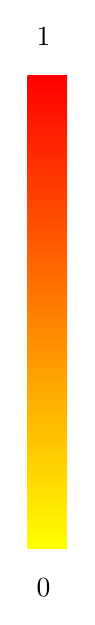
\begin{tikzpicture}[scale=1.0,auto,swap]
    \shade[top color=red,bottom color=yellow] (0,0) rectangle (0.5,6);
    \node[inner sep=0] (corr_text) at (0.2,6.5) {1};
    \node[inner sep=0] (corr_text) at (0.2,-0.5) {0};
  \end{tikzpicture}
  \caption{EBM}
\end{figure}


\begin{figure}[H]
  \centering
  %\begin{subfigure}[b]{0.15\textwidth}
    \begin{tikzpicture}[scale=1.0,auto,swap]

    % the two brain figures on top
    \node (upper_brain) at (0,1.5) { \includegraphics*[scale=\scaleBrainImg,trim=0 0 240 0]{images/GMM/stage_6.eps}};
    \node (lower_brain) at (0,-1.5) { \includegraphics*[scale=\scaleBrainImg,trim=240 0 0 0]{images/GMM/stage_6.eps}};

    % the 6 circles
    \draw[fill=col100] (-1.6,-3.4) circle [radius=0.33cm] node {\scriptsize A};
    \draw[fill=col101] (-0.7,-3.4) circle [radius=0.33cm] node {\scriptsize P};
    \draw[fill=col102] (0.2,-3.4) circle [radius=0.33cm] node {\scriptsize T};
    \draw[fill=col103] (-1.6,-4.2) circle [radius=0.33cm] node {\scriptsize C1};
    \draw[fill=col104] (-0.7,-4.2) circle [radius=0.33cm] node {\scriptsize C2};
    \draw[fill=col105] (0.2,-4.2) circle [radius=0.33cm] node {\scriptsize C3};

    % the big circle on the right
    \draw[fill=col106] (1.3,-3.8) circle [radius=0.6cm] node {\scriptsize FDG};

    \end{tikzpicture}
  %\end{subfigure}
  % next subfigure
  \hspace{-1.5em}
  ~
  %\begin{subfigure}[b]{0.15\textwidth}
    \begin{tikzpicture}[scale=1.0,auto,swap]

    % the two brain figures on top
    \node (upper_brain) at (0,1.5) { \includegraphics*[scale=\scaleBrainImg,trim=0 0 240 0]{images/GMM/stage_12.eps}};
    \node (lower_brain) at (0,-1.5) { \includegraphics*[scale=\scaleBrainImg,trim=240 0 0 0]{images/GMM/stage_12.eps}};

    % the 6 circles
    \draw[fill=col110] (-1.6,-3.4) circle [radius=0.33cm] node {\scriptsize A};
    \draw[fill=col111] (-0.7,-3.4) circle [radius=0.33cm] node {\scriptsize P};
    \draw[fill=col112] (0.2,-3.4) circle [radius=0.33cm] node {\scriptsize T};
    \draw[fill=col113] (-1.6,-4.2) circle [radius=0.33cm] node {\scriptsize C1};
    \draw[fill=col114] (-0.7,-4.2) circle [radius=0.33cm] node {\scriptsize C2};
    \draw[fill=col115] (0.2,-4.2) circle [radius=0.33cm] node {\scriptsize C3};

    % the big circle on the right
    \draw[fill=col116] (1.3,-3.8) circle [radius=0.6cm] node {\scriptsize FDG};

    \end{tikzpicture}
  %\end{subfigure}
  % next subfigure
  \hspace{-1.5em}
  ~
  %\begin{subfigure}[b]{0.15\textwidth}
    \begin{tikzpicture}[scale=1.0,auto,swap]

    % the two brain figures on top
    \node (upper_brain) at (0,1.5) { \includegraphics*[scale=\scaleBrainImg,trim=0 0 240 0]{images/GMM/stage_18.eps}};
    \node (lower_brain) at (0,-1.5) { \includegraphics*[scale=\scaleBrainImg,trim=240 0 0 0]{images/GMM/stage_18.eps}};

    % the 6 circles
    \draw[fill=col120] (-1.6,-3.4) circle [radius=0.33cm] node {\scriptsize A};
    \draw[fill=col121] (-0.7,-3.4) circle [radius=0.33cm] node {\scriptsize P};
    \draw[fill=col122] (0.2,-3.4) circle [radius=0.33cm] node {\scriptsize T};
    \draw[fill=col123] (-1.6,-4.2) circle [radius=0.33cm] node {\scriptsize C1};
    \draw[fill=col124] (-0.7,-4.2) circle [radius=0.33cm] node {\scriptsize C2};
    \draw[fill=col125] (0.2,-4.2) circle [radius=0.33cm] node {\scriptsize C3};

    % the big circle on the right
    \draw[fill=col126] (1.3,-3.8) circle [radius=0.6cm] node {\scriptsize FDG};

    \end{tikzpicture}
  %\end{subfigure}
  % next subfigure
  \hspace{-1.5em}
  ~
  %\begin{subfigure}[b]{0.15\textwidth}
    \begin{tikzpicture}[scale=1.0,auto,swap]

    % the two brain figures on top
    \node (upper_brain) at (0,1.5) { \includegraphics*[scale=\scaleBrainImg,trim=0 0 240 0]{images/GMM/stage_24.eps}};
    \node (lower_brain) at (0,-1.5) { \includegraphics*[scale=\scaleBrainImg,trim=240 0 0 0]{images/GMM/stage_24.eps}};

    % the 6 circles
    \draw[fill=col130] (-1.6,-3.4) circle [radius=0.33cm] node {\scriptsize A};
    \draw[fill=col131] (-0.7,-3.4) circle [radius=0.33cm] node {\scriptsize P};
    \draw[fill=col132] (0.2,-3.4) circle [radius=0.33cm] node {\scriptsize T};
    \draw[fill=col133] (-1.6,-4.2) circle [radius=0.33cm] node {\scriptsize C1};
    \draw[fill=col134] (-0.7,-4.2) circle [radius=0.33cm] node {\scriptsize C2};
    \draw[fill=col135] (0.2,-4.2) circle [radius=0.33cm] node {\scriptsize C3};

    % the big circle on the right
    \draw[fill=col136] (1.3,-3.8) circle [radius=0.6cm] node {\scriptsize FDG};

    \end{tikzpicture}
  %\end{subfigure}
  % next subfigure
  \hspace{-1.5em}
  ~
  %\begin{subfigure}[b]{0.15\textwidth}
    \begin{tikzpicture}[scale=1.0,auto,swap]

    % the two brain figures on top
    \node (upper_brain) at (0,1.5) { \includegraphics*[scale=\scaleBrainImg,trim=0 0 240 0]{images/GMM/stage_36.eps}};
    \node (lower_brain) at (0,-1.5) { \includegraphics*[scale=\scaleBrainImg,trim=240 0 0 0]{images/GMM/stage_36.eps}};

    % the 6 circles
    \draw[fill=col140] (-1.6,-3.4) circle [radius=0.33cm] node {\scriptsize A};
    \draw[fill=col141] (-0.7,-3.4) circle [radius=0.33cm] node {\scriptsize P};
    \draw[fill=col142] (0.2,-3.4) circle [radius=0.33cm] node {\scriptsize T};
    \draw[fill=col143] (-1.6,-4.2) circle [radius=0.33cm] node {\scriptsize C1};
    \draw[fill=col144] (-0.7,-4.2) circle [radius=0.33cm] node {\scriptsize C2};
    \draw[fill=col145] (0.2,-4.2) circle [radius=0.33cm] node {\scriptsize C3};

    % the big circle on the right
    \draw[fill=col146] (1.3,-3.8) circle [radius=0.6cm] node {\scriptsize FDG};

    \end{tikzpicture}
  %\end{subfigure}
  % next subfigure
  \hspace{-1.5em}
  ~
  \hspace{1em}
  % the red-to-yellow gradient on the right 
  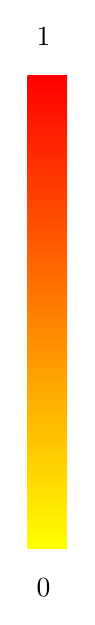
\begin{tikzpicture}[scale=1.0,auto,swap]
    \shade[top color=red,bottom color=yellow] (0,0) rectangle (0.5,6);
    \node[inner sep=0] (corr_text) at (0.2,6.5) {1};
    \node[inner sep=0] (corr_text) at (0.2,-0.5) {0};
  \end{tikzpicture}
  \caption{GMM}
\end{figure}


\begin{figure}[H]
  \centering
  %\begin{subfigure}[b]{0.15\textwidth}
    \begin{tikzpicture}[scale=1.0,auto,swap]

    % the two brain figures on top
    \node (upper_brain) at (0,1.5) { \includegraphics*[scale=\scaleBrainImg,trim=0 0 240 0]{images/cluster1/stage_6.eps}};
    \node (lower_brain) at (0,-1.5) { \includegraphics*[scale=\scaleBrainImg,trim=240 0 0 0]{images/cluster1/stage_6.eps}};

    % the 6 circles
    \draw[fill=col200] (-1.6,-3.4) circle [radius=0.33cm] node {\scriptsize A};
    \draw[fill=col201] (-0.7,-3.4) circle [radius=0.33cm] node {\scriptsize P};
    \draw[fill=col202] (0.2,-3.4) circle [radius=0.33cm] node {\scriptsize T};
    \draw[fill=col203] (-1.6,-4.2) circle [radius=0.33cm] node {\scriptsize C1};
    \draw[fill=col204] (-0.7,-4.2) circle [radius=0.33cm] node {\scriptsize C2};
    \draw[fill=col205] (0.2,-4.2) circle [radius=0.33cm] node {\scriptsize C3};

    % the big circle on the right
    \draw[fill=col206] (1.3,-3.8) circle [radius=0.6cm] node {\scriptsize FDG};

    \end{tikzpicture}
  %\end{subfigure}
  % next subfigure
  \hspace{-1.5em}
  ~
  %\begin{subfigure}[b]{0.15\textwidth}
    \begin{tikzpicture}[scale=1.0,auto,swap]

    % the two brain figures on top
    \node (upper_brain) at (0,1.5) { \includegraphics*[scale=\scaleBrainImg,trim=0 0 240 0]{images/cluster1/stage_12.eps}};
    \node (lower_brain) at (0,-1.5) { \includegraphics*[scale=\scaleBrainImg,trim=240 0 0 0]{images/cluster1/stage_12.eps}};

    % the 6 circles
    \draw[fill=col210] (-1.6,-3.4) circle [radius=0.33cm] node {\scriptsize A};
    \draw[fill=col211] (-0.7,-3.4) circle [radius=0.33cm] node {\scriptsize P};
    \draw[fill=col212] (0.2,-3.4) circle [radius=0.33cm] node {\scriptsize T};
    \draw[fill=col213] (-1.6,-4.2) circle [radius=0.33cm] node {\scriptsize C1};
    \draw[fill=col214] (-0.7,-4.2) circle [radius=0.33cm] node {\scriptsize C2};
    \draw[fill=col215] (0.2,-4.2) circle [radius=0.33cm] node {\scriptsize C3};

    % the big circle on the right
    \draw[fill=col216] (1.3,-3.8) circle [radius=0.6cm] node {\scriptsize FDG};

    \end{tikzpicture}
  %\end{subfigure}
  % next subfigure
  \hspace{-1.5em}
  ~
  %\begin{subfigure}[b]{0.15\textwidth}
    \begin{tikzpicture}[scale=1.0,auto,swap]

    % the two brain figures on top
    \node (upper_brain) at (0,1.5) { \includegraphics*[scale=\scaleBrainImg,trim=0 0 240 0]{images/cluster1/stage_18.eps}};
    \node (lower_brain) at (0,-1.5) { \includegraphics*[scale=\scaleBrainImg,trim=240 0 0 0]{images/cluster1/stage_18.eps}};

    % the 6 circles
    \draw[fill=col220] (-1.6,-3.4) circle [radius=0.33cm] node {\scriptsize A};
    \draw[fill=col221] (-0.7,-3.4) circle [radius=0.33cm] node {\scriptsize P};
    \draw[fill=col222] (0.2,-3.4) circle [radius=0.33cm] node {\scriptsize T};
    \draw[fill=col223] (-1.6,-4.2) circle [radius=0.33cm] node {\scriptsize C1};
    \draw[fill=col224] (-0.7,-4.2) circle [radius=0.33cm] node {\scriptsize C2};
    \draw[fill=col225] (0.2,-4.2) circle [radius=0.33cm] node {\scriptsize C3};

    % the big circle on the right
    \draw[fill=col226] (1.3,-3.8) circle [radius=0.6cm] node {\scriptsize FDG};

    \end{tikzpicture}
  %\end{subfigure}
  % next subfigure
  \hspace{-1.5em}
  ~
  %\begin{subfigure}[b]{0.15\textwidth}
    \begin{tikzpicture}[scale=1.0,auto,swap]

    % the two brain figures on top
    \node (upper_brain) at (0,1.5) { \includegraphics*[scale=\scaleBrainImg,trim=0 0 240 0]{images/cluster1/stage_24.eps}};
    \node (lower_brain) at (0,-1.5) { \includegraphics*[scale=\scaleBrainImg,trim=240 0 0 0]{images/cluster1/stage_24.eps}};

    % the 6 circles
    \draw[fill=col230] (-1.6,-3.4) circle [radius=0.33cm] node {\scriptsize A};
    \draw[fill=col231] (-0.7,-3.4) circle [radius=0.33cm] node {\scriptsize P};
    \draw[fill=col232] (0.2,-3.4) circle [radius=0.33cm] node {\scriptsize T};
    \draw[fill=col233] (-1.6,-4.2) circle [radius=0.33cm] node {\scriptsize C1};
    \draw[fill=col234] (-0.7,-4.2) circle [radius=0.33cm] node {\scriptsize C2};
    \draw[fill=col235] (0.2,-4.2) circle [radius=0.33cm] node {\scriptsize C3};

    % the big circle on the right
    \draw[fill=col236] (1.3,-3.8) circle [radius=0.6cm] node {\scriptsize FDG};

    \end{tikzpicture}
  %\end{subfigure}
  % next subfigure
  \hspace{-1.5em}
  ~
  %\begin{subfigure}[b]{0.15\textwidth}
    \begin{tikzpicture}[scale=1.0,auto,swap]

    % the two brain figures on top
    \node (upper_brain) at (0,1.5) { \includegraphics*[scale=\scaleBrainImg,trim=0 0 240 0]{images/cluster1/stage_36.eps}};
    \node (lower_brain) at (0,-1.5) { \includegraphics*[scale=\scaleBrainImg,trim=240 0 0 0]{images/cluster1/stage_36.eps}};

    % the 6 circles
    \draw[fill=col240] (-1.6,-3.4) circle [radius=0.33cm] node {\scriptsize A};
    \draw[fill=col241] (-0.7,-3.4) circle [radius=0.33cm] node {\scriptsize P};
    \draw[fill=col242] (0.2,-3.4) circle [radius=0.33cm] node {\scriptsize T};
    \draw[fill=col243] (-1.6,-4.2) circle [radius=0.33cm] node {\scriptsize C1};
    \draw[fill=col244] (-0.7,-4.2) circle [radius=0.33cm] node {\scriptsize C2};
    \draw[fill=col245] (0.2,-4.2) circle [radius=0.33cm] node {\scriptsize C3};

    % the big circle on the right
    \draw[fill=col246] (1.3,-3.8) circle [radius=0.6cm] node {\scriptsize FDG};

    \end{tikzpicture}
  %\end{subfigure}
  % next subfigure
  \hspace{-1.5em}
  ~
  \hspace{1em}
  % the red-to-yellow gradient on the right 
  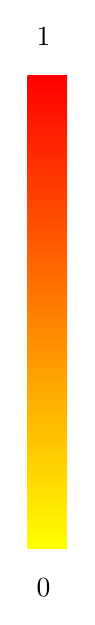
\begin{tikzpicture}[scale=1.0,auto,swap]
    \shade[top color=red,bottom color=yellow] (0,0) rectangle (0.5,6);
    \node[inner sep=0] (corr_text) at (0.2,6.5) {1};
    \node[inner sep=0] (corr_text) at (0.2,-0.5) {0};
  \end{tikzpicture}
  \caption{cluster1}
\end{figure}


\begin{figure}[H]
  \centering
  %\begin{subfigure}[b]{0.15\textwidth}
    \begin{tikzpicture}[scale=1.0,auto,swap]

    % the two brain figures on top
    \node (upper_brain) at (0,1.5) { \includegraphics*[scale=\scaleBrainImg,trim=0 0 240 0]{images/cluster2/stage_6.eps}};
    \node (lower_brain) at (0,-1.5) { \includegraphics*[scale=\scaleBrainImg,trim=240 0 0 0]{images/cluster2/stage_6.eps}};

    % the 6 circles
    \draw[fill=col300] (-1.6,-3.4) circle [radius=0.33cm] node {\scriptsize A};
    \draw[fill=col301] (-0.7,-3.4) circle [radius=0.33cm] node {\scriptsize P};
    \draw[fill=col302] (0.2,-3.4) circle [radius=0.33cm] node {\scriptsize T};
    \draw[fill=col303] (-1.6,-4.2) circle [radius=0.33cm] node {\scriptsize C1};
    \draw[fill=col304] (-0.7,-4.2) circle [radius=0.33cm] node {\scriptsize C2};
    \draw[fill=col305] (0.2,-4.2) circle [radius=0.33cm] node {\scriptsize C3};

    % the big circle on the right
    \draw[fill=col306] (1.3,-3.8) circle [radius=0.6cm] node {\scriptsize FDG};

    \end{tikzpicture}
  %\end{subfigure}
  % next subfigure
  \hspace{-1.5em}
  ~
  %\begin{subfigure}[b]{0.15\textwidth}
    \begin{tikzpicture}[scale=1.0,auto,swap]

    % the two brain figures on top
    \node (upper_brain) at (0,1.5) { \includegraphics*[scale=\scaleBrainImg,trim=0 0 240 0]{images/cluster2/stage_12.eps}};
    \node (lower_brain) at (0,-1.5) { \includegraphics*[scale=\scaleBrainImg,trim=240 0 0 0]{images/cluster2/stage_12.eps}};

    % the 6 circles
    \draw[fill=col310] (-1.6,-3.4) circle [radius=0.33cm] node {\scriptsize A};
    \draw[fill=col311] (-0.7,-3.4) circle [radius=0.33cm] node {\scriptsize P};
    \draw[fill=col312] (0.2,-3.4) circle [radius=0.33cm] node {\scriptsize T};
    \draw[fill=col313] (-1.6,-4.2) circle [radius=0.33cm] node {\scriptsize C1};
    \draw[fill=col314] (-0.7,-4.2) circle [radius=0.33cm] node {\scriptsize C2};
    \draw[fill=col315] (0.2,-4.2) circle [radius=0.33cm] node {\scriptsize C3};

    % the big circle on the right
    \draw[fill=col316] (1.3,-3.8) circle [radius=0.6cm] node {\scriptsize FDG};

    \end{tikzpicture}
  %\end{subfigure}
  % next subfigure
  \hspace{-1.5em}
  ~
  %\begin{subfigure}[b]{0.15\textwidth}
    \begin{tikzpicture}[scale=1.0,auto,swap]

    % the two brain figures on top
    \node (upper_brain) at (0,1.5) { \includegraphics*[scale=\scaleBrainImg,trim=0 0 240 0]{images/cluster2/stage_18.eps}};
    \node (lower_brain) at (0,-1.5) { \includegraphics*[scale=\scaleBrainImg,trim=240 0 0 0]{images/cluster2/stage_18.eps}};

    % the 6 circles
    \draw[fill=col320] (-1.6,-3.4) circle [radius=0.33cm] node {\scriptsize A};
    \draw[fill=col321] (-0.7,-3.4) circle [radius=0.33cm] node {\scriptsize P};
    \draw[fill=col322] (0.2,-3.4) circle [radius=0.33cm] node {\scriptsize T};
    \draw[fill=col323] (-1.6,-4.2) circle [radius=0.33cm] node {\scriptsize C1};
    \draw[fill=col324] (-0.7,-4.2) circle [radius=0.33cm] node {\scriptsize C2};
    \draw[fill=col325] (0.2,-4.2) circle [radius=0.33cm] node {\scriptsize C3};

    % the big circle on the right
    \draw[fill=col326] (1.3,-3.8) circle [radius=0.6cm] node {\scriptsize FDG};

    \end{tikzpicture}
  %\end{subfigure}
  % next subfigure
  \hspace{-1.5em}
  ~
  %\begin{subfigure}[b]{0.15\textwidth}
    \begin{tikzpicture}[scale=1.0,auto,swap]

    % the two brain figures on top
    \node (upper_brain) at (0,1.5) { \includegraphics*[scale=\scaleBrainImg,trim=0 0 240 0]{images/cluster2/stage_24.eps}};
    \node (lower_brain) at (0,-1.5) { \includegraphics*[scale=\scaleBrainImg,trim=240 0 0 0]{images/cluster2/stage_24.eps}};

    % the 6 circles
    \draw[fill=col330] (-1.6,-3.4) circle [radius=0.33cm] node {\scriptsize A};
    \draw[fill=col331] (-0.7,-3.4) circle [radius=0.33cm] node {\scriptsize P};
    \draw[fill=col332] (0.2,-3.4) circle [radius=0.33cm] node {\scriptsize T};
    \draw[fill=col333] (-1.6,-4.2) circle [radius=0.33cm] node {\scriptsize C1};
    \draw[fill=col334] (-0.7,-4.2) circle [radius=0.33cm] node {\scriptsize C2};
    \draw[fill=col335] (0.2,-4.2) circle [radius=0.33cm] node {\scriptsize C3};

    % the big circle on the right
    \draw[fill=col336] (1.3,-3.8) circle [radius=0.6cm] node {\scriptsize FDG};

    \end{tikzpicture}
  %\end{subfigure}
  % next subfigure
  \hspace{-1.5em}
  ~
  %\begin{subfigure}[b]{0.15\textwidth}
    \begin{tikzpicture}[scale=1.0,auto,swap]

    % the two brain figures on top
    \node (upper_brain) at (0,1.5) { \includegraphics*[scale=\scaleBrainImg,trim=0 0 240 0]{images/cluster2/stage_36.eps}};
    \node (lower_brain) at (0,-1.5) { \includegraphics*[scale=\scaleBrainImg,trim=240 0 0 0]{images/cluster2/stage_36.eps}};

    % the 6 circles
    \draw[fill=col340] (-1.6,-3.4) circle [radius=0.33cm] node {\scriptsize A};
    \draw[fill=col341] (-0.7,-3.4) circle [radius=0.33cm] node {\scriptsize P};
    \draw[fill=col342] (0.2,-3.4) circle [radius=0.33cm] node {\scriptsize T};
    \draw[fill=col343] (-1.6,-4.2) circle [radius=0.33cm] node {\scriptsize C1};
    \draw[fill=col344] (-0.7,-4.2) circle [radius=0.33cm] node {\scriptsize C2};
    \draw[fill=col345] (0.2,-4.2) circle [radius=0.33cm] node {\scriptsize C3};

    % the big circle on the right
    \draw[fill=col346] (1.3,-3.8) circle [radius=0.6cm] node {\scriptsize FDG};

    \end{tikzpicture}
  %\end{subfigure}
  % next subfigure
  \hspace{-1.5em}
  ~
  \hspace{1em}
  % the red-to-yellow gradient on the right 
  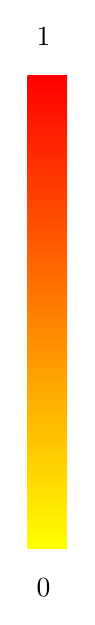
\begin{tikzpicture}[scale=1.0,auto,swap]
    \shade[top color=red,bottom color=yellow] (0,0) rectangle (0.5,6);
    \node[inner sep=0] (corr_text) at (0.2,6.5) {1};
    \node[inner sep=0] (corr_text) at (0.2,-0.5) {0};
  \end{tikzpicture}
  \caption{cluster2}
\end{figure}


\begin{figure}[H]
  \centering
  %\begin{subfigure}[b]{0.15\textwidth}
    \begin{tikzpicture}[scale=1.0,auto,swap]

    % the two brain figures on top
    \node (upper_brain) at (0,1.5) { \includegraphics*[scale=\scaleBrainImg,trim=0 0 240 0]{images/cluster3/stage_6.eps}};
    \node (lower_brain) at (0,-1.5) { \includegraphics*[scale=\scaleBrainImg,trim=240 0 0 0]{images/cluster3/stage_6.eps}};

    % the 6 circles
    \draw[fill=col400] (-1.6,-3.4) circle [radius=0.33cm] node {\scriptsize A};
    \draw[fill=col401] (-0.7,-3.4) circle [radius=0.33cm] node {\scriptsize P};
    \draw[fill=col402] (0.2,-3.4) circle [radius=0.33cm] node {\scriptsize T};
    \draw[fill=col403] (-1.6,-4.2) circle [radius=0.33cm] node {\scriptsize C1};
    \draw[fill=col404] (-0.7,-4.2) circle [radius=0.33cm] node {\scriptsize C2};
    \draw[fill=col405] (0.2,-4.2) circle [radius=0.33cm] node {\scriptsize C3};

    % the big circle on the right
    \draw[fill=col406] (1.3,-3.8) circle [radius=0.6cm] node {\scriptsize FDG};

    \end{tikzpicture}
  %\end{subfigure}
  % next subfigure
  \hspace{-1.5em}
  ~
  %\begin{subfigure}[b]{0.15\textwidth}
    \begin{tikzpicture}[scale=1.0,auto,swap]

    % the two brain figures on top
    \node (upper_brain) at (0,1.5) { \includegraphics*[scale=\scaleBrainImg,trim=0 0 240 0]{images/cluster3/stage_12.eps}};
    \node (lower_brain) at (0,-1.5) { \includegraphics*[scale=\scaleBrainImg,trim=240 0 0 0]{images/cluster3/stage_12.eps}};

    % the 6 circles
    \draw[fill=col410] (-1.6,-3.4) circle [radius=0.33cm] node {\scriptsize A};
    \draw[fill=col411] (-0.7,-3.4) circle [radius=0.33cm] node {\scriptsize P};
    \draw[fill=col412] (0.2,-3.4) circle [radius=0.33cm] node {\scriptsize T};
    \draw[fill=col413] (-1.6,-4.2) circle [radius=0.33cm] node {\scriptsize C1};
    \draw[fill=col414] (-0.7,-4.2) circle [radius=0.33cm] node {\scriptsize C2};
    \draw[fill=col415] (0.2,-4.2) circle [radius=0.33cm] node {\scriptsize C3};

    % the big circle on the right
    \draw[fill=col416] (1.3,-3.8) circle [radius=0.6cm] node {\scriptsize FDG};

    \end{tikzpicture}
  %\end{subfigure}
  % next subfigure
  \hspace{-1.5em}
  ~
  %\begin{subfigure}[b]{0.15\textwidth}
    \begin{tikzpicture}[scale=1.0,auto,swap]

    % the two brain figures on top
    \node (upper_brain) at (0,1.5) { \includegraphics*[scale=\scaleBrainImg,trim=0 0 240 0]{images/cluster3/stage_18.eps}};
    \node (lower_brain) at (0,-1.5) { \includegraphics*[scale=\scaleBrainImg,trim=240 0 0 0]{images/cluster3/stage_18.eps}};

    % the 6 circles
    \draw[fill=col420] (-1.6,-3.4) circle [radius=0.33cm] node {\scriptsize A};
    \draw[fill=col421] (-0.7,-3.4) circle [radius=0.33cm] node {\scriptsize P};
    \draw[fill=col422] (0.2,-3.4) circle [radius=0.33cm] node {\scriptsize T};
    \draw[fill=col423] (-1.6,-4.2) circle [radius=0.33cm] node {\scriptsize C1};
    \draw[fill=col424] (-0.7,-4.2) circle [radius=0.33cm] node {\scriptsize C2};
    \draw[fill=col425] (0.2,-4.2) circle [radius=0.33cm] node {\scriptsize C3};

    % the big circle on the right
    \draw[fill=col426] (1.3,-3.8) circle [radius=0.6cm] node {\scriptsize FDG};

    \end{tikzpicture}
  %\end{subfigure}
  % next subfigure
  \hspace{-1.5em}
  ~
  %\begin{subfigure}[b]{0.15\textwidth}
    \begin{tikzpicture}[scale=1.0,auto,swap]

    % the two brain figures on top
    \node (upper_brain) at (0,1.5) { \includegraphics*[scale=\scaleBrainImg,trim=0 0 240 0]{images/cluster3/stage_24.eps}};
    \node (lower_brain) at (0,-1.5) { \includegraphics*[scale=\scaleBrainImg,trim=240 0 0 0]{images/cluster3/stage_24.eps}};

    % the 6 circles
    \draw[fill=col430] (-1.6,-3.4) circle [radius=0.33cm] node {\scriptsize A};
    \draw[fill=col431] (-0.7,-3.4) circle [radius=0.33cm] node {\scriptsize P};
    \draw[fill=col432] (0.2,-3.4) circle [radius=0.33cm] node {\scriptsize T};
    \draw[fill=col433] (-1.6,-4.2) circle [radius=0.33cm] node {\scriptsize C1};
    \draw[fill=col434] (-0.7,-4.2) circle [radius=0.33cm] node {\scriptsize C2};
    \draw[fill=col435] (0.2,-4.2) circle [radius=0.33cm] node {\scriptsize C3};

    % the big circle on the right
    \draw[fill=col436] (1.3,-3.8) circle [radius=0.6cm] node {\scriptsize FDG};

    \end{tikzpicture}
  %\end{subfigure}
  % next subfigure
  \hspace{-1.5em}
  ~
  %\begin{subfigure}[b]{0.15\textwidth}
    \begin{tikzpicture}[scale=1.0,auto,swap]

    % the two brain figures on top
    \node (upper_brain) at (0,1.5) { \includegraphics*[scale=\scaleBrainImg,trim=0 0 240 0]{images/cluster3/stage_36.eps}};
    \node (lower_brain) at (0,-1.5) { \includegraphics*[scale=\scaleBrainImg,trim=240 0 0 0]{images/cluster3/stage_36.eps}};

    % the 6 circles
    \draw[fill=col440] (-1.6,-3.4) circle [radius=0.33cm] node {\scriptsize A};
    \draw[fill=col441] (-0.7,-3.4) circle [radius=0.33cm] node {\scriptsize P};
    \draw[fill=col442] (0.2,-3.4) circle [radius=0.33cm] node {\scriptsize T};
    \draw[fill=col443] (-1.6,-4.2) circle [radius=0.33cm] node {\scriptsize C1};
    \draw[fill=col444] (-0.7,-4.2) circle [radius=0.33cm] node {\scriptsize C2};
    \draw[fill=col445] (0.2,-4.2) circle [radius=0.33cm] node {\scriptsize C3};

    % the big circle on the right
    \draw[fill=col446] (1.3,-3.8) circle [radius=0.6cm] node {\scriptsize FDG};

    \end{tikzpicture}
  %\end{subfigure}
  % next subfigure
  \hspace{-1.5em}
  ~
  \hspace{1em}
  % the red-to-yellow gradient on the right 
  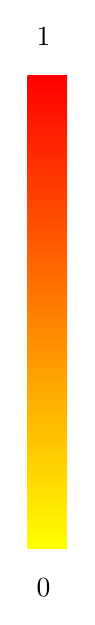
\begin{tikzpicture}[scale=1.0,auto,swap]
    \shade[top color=red,bottom color=yellow] (0,0) rectangle (0.5,6);
    \node[inner sep=0] (corr_text) at (0.2,6.5) {1};
    \node[inner sep=0] (corr_text) at (0.2,-0.5) {0};
  \end{tikzpicture}
  \caption{cluster3}
\end{figure}



% scale parameter for the font size in the circles
\newcommand*{\scaleLabelImg}{0.7}
\begin{figure}[H]
  \centering
  {\scalefont{\scaleLabelImg}
  \begin{tikzpicture}[scale=1.0,auto,swap]

  % the two brain figures on top
  \node (brain) at (0,1.5) { \includegraphics*[scale=\scaleLabelImg]{images/Mid-Lateral_surface3.eps}};

  % the 6 circles
  \draw[scale=\scaleLabelImg] (-9,-6) circle [radius=2cm] node {ABETA142};
  \draw[scale=\scaleLabelImg] (-4,-6) circle [radius=2cm] node {PTAU181P};
  \draw[scale=\scaleLabelImg] (1,-6) circle [radius=2cm] node {TAU};
  \draw[scale=\scaleLabelImg] (-9,-10.5) circle [radius=2cm] node {RAVLT};
  \draw[scale=\scaleLabelImg] (-4,-10.5) circle [radius=2cm] node {MMSE};
  \draw[scale=\scaleLabelImg] (1,-10.5) circle [radius=2cm] node {ADAS13};

  % the big circle on the right
  \draw[scale=\scaleLabelImg] (8,-8.25) circle [radius=4cm] node {FDG-PET};

  \end{tikzpicture}
  }

  \caption{Labels of the different areas analysed}
\end{figure}

\end{document}

